\newpage
\section{Top Level}

\subsection{Introduction}

In this section, we integrate all previously explained design elements to create a unified single-cycle processor. The top-level module includes specific multiplexers labeled as M1, M2, and M3. M1 controls the datapath for the second operand of the ALU, M2 manages the write-back operation to the register file, and M3 adjusts the datapath of the PC register during flash operations. These multiplexers are crucial as they enable the processor to adapt its datapaths based on the instruction being executed, allowing a variety of operations to be performed. We will also understand the instruction memory flash mechanism in detail.
\\ 
\hfill \break
This section focuses on implementing the single-cycle processor's datapath flow described in the product overview. It will detail how different instruction classes are executed, emphasizing the role of these multiplexers in enabling diverse operations within the processor.
\begin{itemize}
  \item Datapath for R-Type instructions.
  \item Datapath for load/store instructions.
  \item Datapath for branch-if-equal instruction.
\end{itemize}

\subsection{Datapath for R-Type instructions}

The figure below shows the datapath operation (Highlighted in red) for an R-type instruction such as \texttt{add x1, x2, x3}. Although everything occurs in one clock cycle, we can think of several steps to execute the instruction.

\begin{figure}[H]
    \centering
    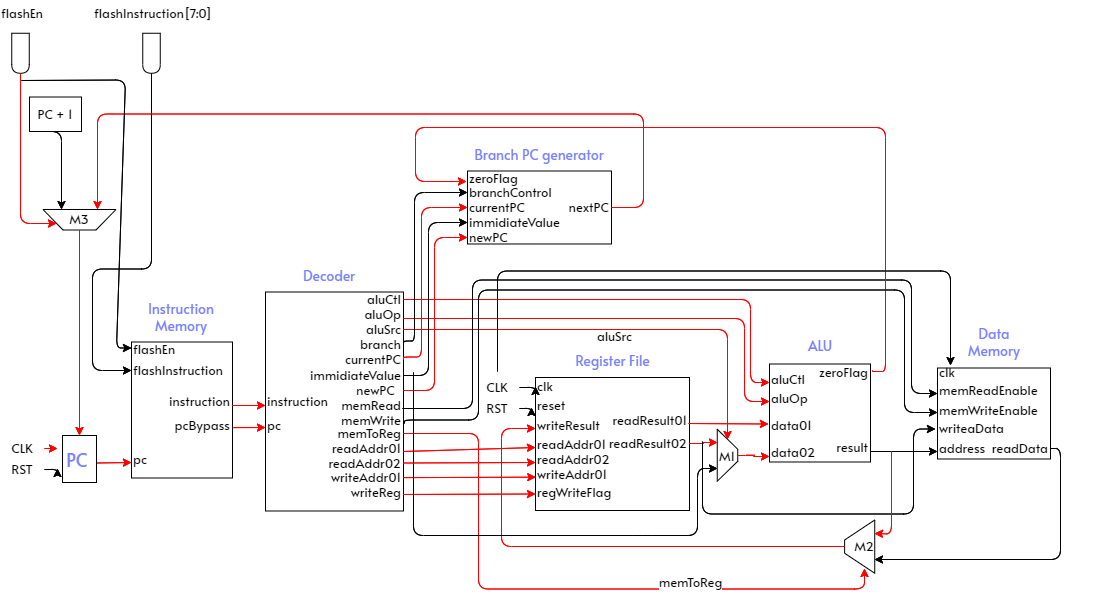
\includegraphics[width=0.95\textwidth, height=0.4\textheight]{Image/01_Rtype.png}
    \caption{R-Type Datapath}
    \label{fig:R-Type Datapath}
\end{figure}


\begin{itemize}
  \item On each rising edge of the clock pulse, if the processor is not in flash mode (flashEn is zero), the PC increments by 4.
  \item The instruction located at the updated PC (oldPC + 4) is fetched from the instruction memory and sent to the decoder for decoding. This process generates necessary signals and addresses required for executing the instruction.
  \item  For the current instruction "add x1, x2, x3", values from register file addresses x2 and x3 are fetched and sent to the ALU.

  \item  As "add" is an R-Type instruction, aluSrc signal is zero, and M1 mux directs readResult02 to the ALU as the second operand.
  \item The ALU performs an arithmetic addition based on signals aluCtl and aluOp from the decoder. The resulting value is written back to register file location x1. memToReg flag is zero, and regWriteFlag is High, enabling this write operation.

  \item Since the branch signal is zero, the branch PC generator forwards the newPC (oldPC + 4) to nextPC. This updated value is loaded into the PC register at the next rising edge of the clock cycle.
\end{itemize}


\subsection{Datapath for load/store instructions}

The figure below shows the datapath operation (Highlighted in red) for a load instruction such as \texttt{ld x1, offset(x2)}. Although everything occurs in one clock cycle, we can think of several steps to execute the instruction.

\begin{figure}[H]
    \centering
    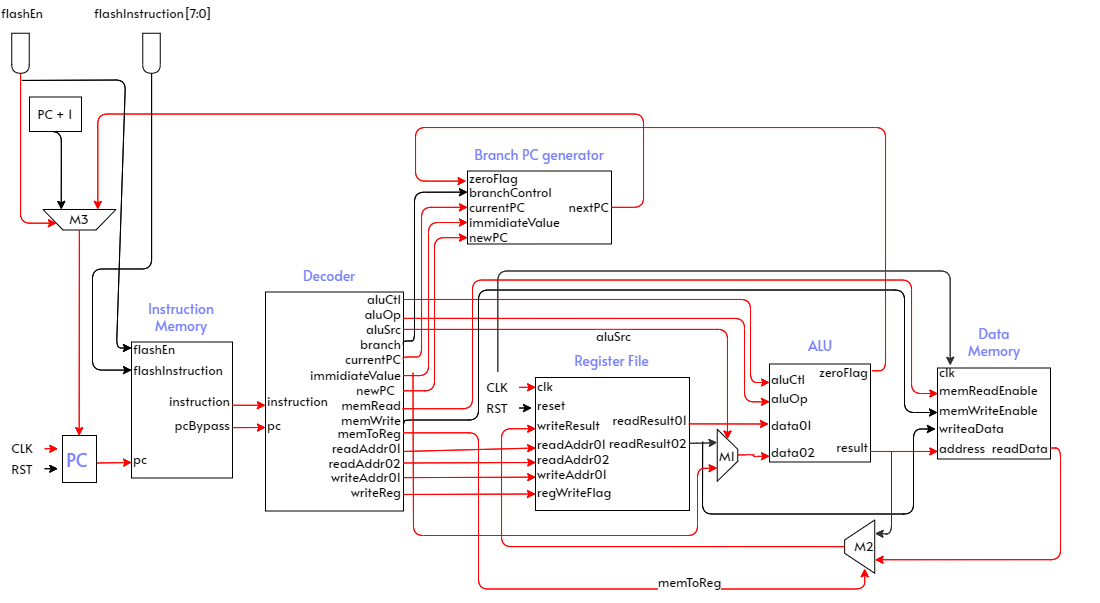
\includegraphics[width=0.95\textwidth, height=0.4\textheight]{Image/02_load.png}
    \caption{load/ store Datapath}
    \label{fig:load/ store Datapath}
\end{figure}

\begin{itemize}
  \item At each rising edge of the clock pulse, the PC increments by 4 when the processor is not in flash mode (flashEn is zero).
  \item The instruction located at the new PC (oldPC + 4) is fetched from the instruction memory and passed to the decoder for decoding. This process generates the necessary signals and addresses required for executing the instruction.

  \item For the current instruction "ld x1, offset(x2)", the value from register file address x2 is sent to the ALU. The ALU's second operand is a 12-bit immediateValue from the decoder, as aluSrc signal is High, and mux M1 adjusts the datapath accordingly compared to the previous instruction.

  \item The ALU adds these operands as directed by signals aluCtl and aluOp, producing the memory address from which data needs to be fetched.

  \item Since the memory read operation is clock-independent, the fetched data is written back to the register file during the falling edge of the same clock cycle. Here, mux M2 alters the datapath for the write-back operation to the register file, since memToReg signal is High. The fetched value is stored in register x1 of the register file.

  \item Meanwhile, with branch signal at zero, the branch PC generator forwards newPC to nextPC (oldPC + 4). This updated value is loaded into the PC register at the next clock cycle's rising edge.
\end{itemize}

Store operations will also have an almost similar datapath to store data from the reg file into the data memory.

\subsection{Datapath for branch-if-equal instructions}

The figure below shows the datapath operation (Highlighted in red) for a branch-if-equal instruction such as \texttt{beq x1, x2, offset}. It operates much like an R-format instruction but the ALU output is used to determine whether the PC is written with PC + 4 or the branch target address. Although everything occurs in one clock cycle, we can think of several steps to execute the instruction.


\begin{itemize}
  \item  During each rising edge of the clock pulse, the PC increments by 4 when the processor is not in flash mode (flashEn is zero).
  \item The instruction located at the updated PC (oldPC + 4) is fetched from the instruction memory and forwarded to the decoder for decoding. This step generates the necessary signals and addresses required to execute the instruction.

  \item Two registers, x1 and x2, are accessed and read from the register file.
  \item The ALU subtracts one data value from another, both obtained from the register file. If the result of this operation is zero, the zeroFlag is set High. If the branch flag is also High, indicating a branch instruction, the branch PC generator computes the branch target address by adding the current PC value to the sign-extended immediateValue (offset) extracted from the instruction (12 bits, left shifted by one).
  \item The new branch target address is written into the PC register during the rising edge of the next clock cycle. The instruction memory then retrieves and executes the instruction located at this branch target address. This process occurs independently of the clock due to the nature of instruction memory read operations.
\end{itemize}

\begin{figure}[H]
    \centering
    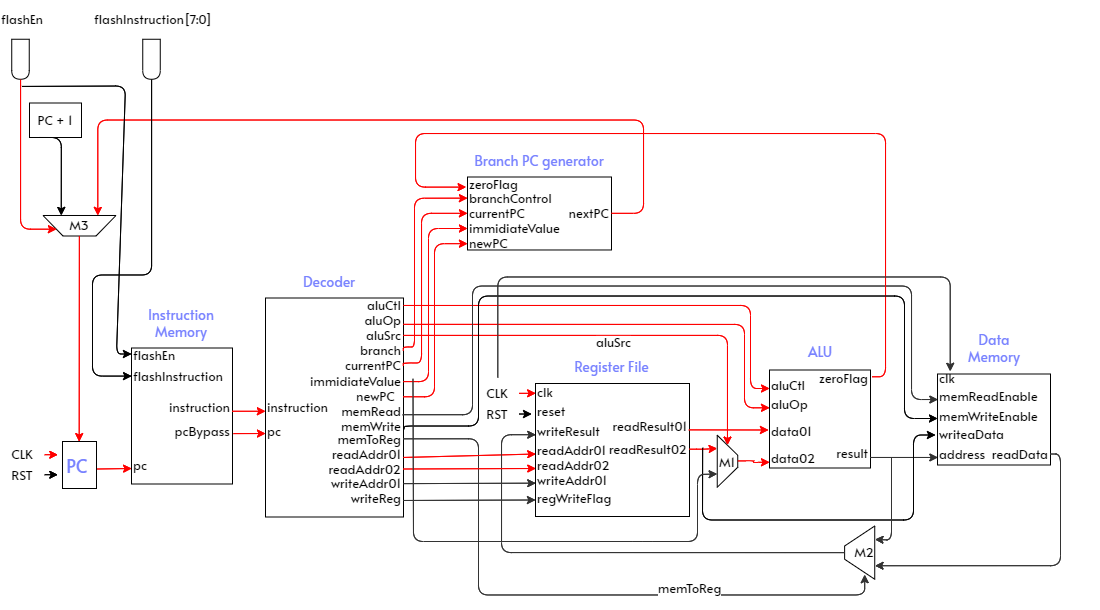
\includegraphics[width=0.95\textwidth, height=0.4\textheight]{Image/03_beq.png}
    \caption{Branch-if-equal Datapath}
    \label{fig:Branch-if-equal Datapath}
\end{figure}

These operations encompass all potential datapaths the processor can generate, providing a comprehensive understanding of the functional principles underlying the single-cycle RISC-V processor.


\subsection{Datapath for processor flash operation}

The diagram below illustrates the datapath operation (highlighted in red) for the processor's instruction memory during a flash operation. In the RISC-V architecture, each instruction is 32 bits wide, while the instruction memory operates on a byte-addressable basis. Initially, a hex file must be generated from high-level languages or assembly code using a dedicated toolchain. Once this hex file is prepared, the processor can be flashed by simulating the process typically handled by an onboard debugger like JTAG or a TAP Controller.
\\ 
\hfill \break
In this scenario, although no specific debugger is employed, the process involves writing one byte at the corresponding PC location in the instruction memory from the hex file. If the flashEn signal is High, the PC increments by one at the rising edge of each clock cycle, enabling the loading of one byte of instruction per clock cycle.

\begin{figure}[H]
    \centering
    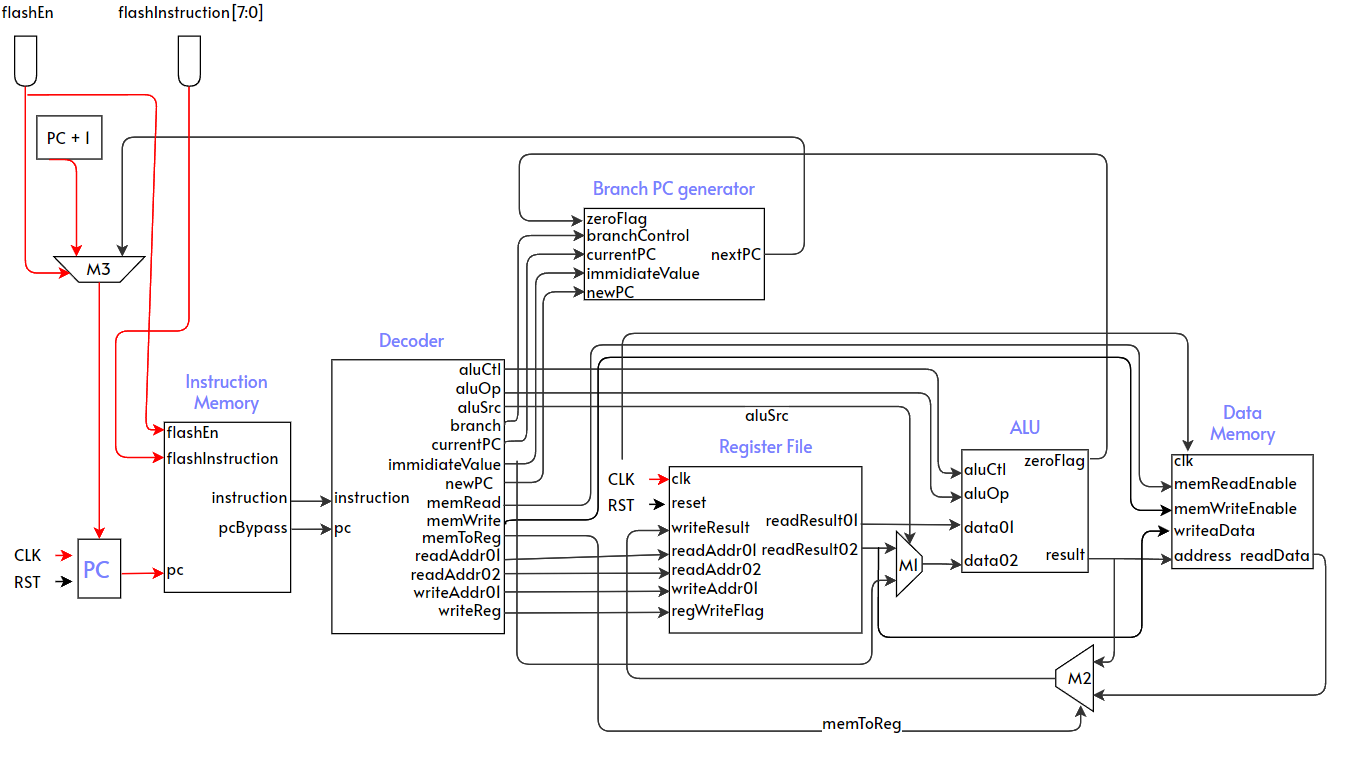
\includegraphics[width=0.95\textwidth, height=0.4\textheight]{Image/04_flash.png}
    \caption{Flash Datapath}
    \label{fig:Flash Datapath}
\end{figure}

After completing the flashing operation, deactivate the flashEn signal and reset the processor. Subsequently, the processor will transition to normal mode and begin executing the instructions stored in the instruction memory that were loaded during the flashing process.

